\documentclass[journal]{IEEEtran}
\usepackage{amsmath,amssymb,amsfonts}
\usepackage{graphicx}
\usepackage{cite}
\usepackage{algorithm}
\usepackage{algorithmic}
\usepackage{booktabs}
\usepackage{multirow}
\usepackage{pifont}
\usepackage{color}
\usepackage{hyperref}
\usepackage{amsthm}

% Placeholder command for TODO notes
\newcommand{\todo}[1]{\textcolor{red}{[TODO: #1]}}

\newtheorem{proposition}{Proposition}

\begin{document}
\title{DV-SLAM: Confidence-Aware LiDAR-Inertial Odometry\\for Sparse Mobile dToF Sensors}

\author{First Author,~\IEEEmembership{Student Member,~IEEE,}
        Second Author,~\IEEEmembership{Member,~IEEE,}
        and~Third Author%
\thanks{This work was supported by \todo{funding info}.}
\thanks{First Author is with the Department of \todo{dept}, \todo{University}, \todo{City}, \todo{Country} (e-mail: \todo{email}).}
\thanks{Second Author is with \todo{affiliation}.}
\thanks{Manuscript received \todo{date}; revised \todo{date}.}}

\markboth{IEEE Robotics and Automation Letters. Preprint Version.}%
{Author \MakeLowercase{\textit{et al.}}: DV-SLAM}

\maketitle

\begin{abstract}
Existing LiDAR-inertial odometry (LIO) systems assume dense point clouds ($>$10K points/scan) with uniform quality. Consumer dToF LiDAR produces only 200--500 usable points per frame, yet no open LIO system operates in this regime. We present DV-SLAM, a camera-free tightly-coupled LIO system designed for this regime. DV-SLAM exploits per-pixel confidence metadata, a discrete quality signal unique to dToF hardware, through multi-level gating at the point, voxel, and observation levels. A Gauss--Markov analysis shows that uniform weighting inflates pose variance by ${\sim}$54\%; a practical two-level approximation recovers most of this gain. The pipeline runs in real time (${\sim}$13\,ms/keyframe) on a mobile processor with no external dependencies beyond Eigen. Against dense-LiDAR ground truth, confidence-aware processing closes much of the quality gap between a consumer dToF sensor and dedicated scanning hardware, approaching the platform's built-in visual-inertial reconstruction in map quality without requiring camera input. We provide the first point-count sweep characterizing the minimum viable observation count for stable LIO on sparse dToF data.
\end{abstract}

\begin{IEEEkeywords}
LiDAR-inertial odometry, direct time-of-flight, mobile 3D scanning, confidence-aware SLAM, error-state Kalman filter.
\end{IEEEkeywords}

%% ============================================================
\section{Introduction}
\label{sec:intro}
%% ============================================================

%% P1: Dense LIO works well
\IEEEPARstart{S}{ystems} such as FAST-LIO2~\cite{xu2022fastlio2} and DLIO~\cite{chen2023dlio} routinely achieve centimeter-level trajectory estimation on mechanical scanning LiDARs producing 10K+ points per scan, where every measured point can be treated as equally reliable.

\begin{figure*}[t]
    \centering
    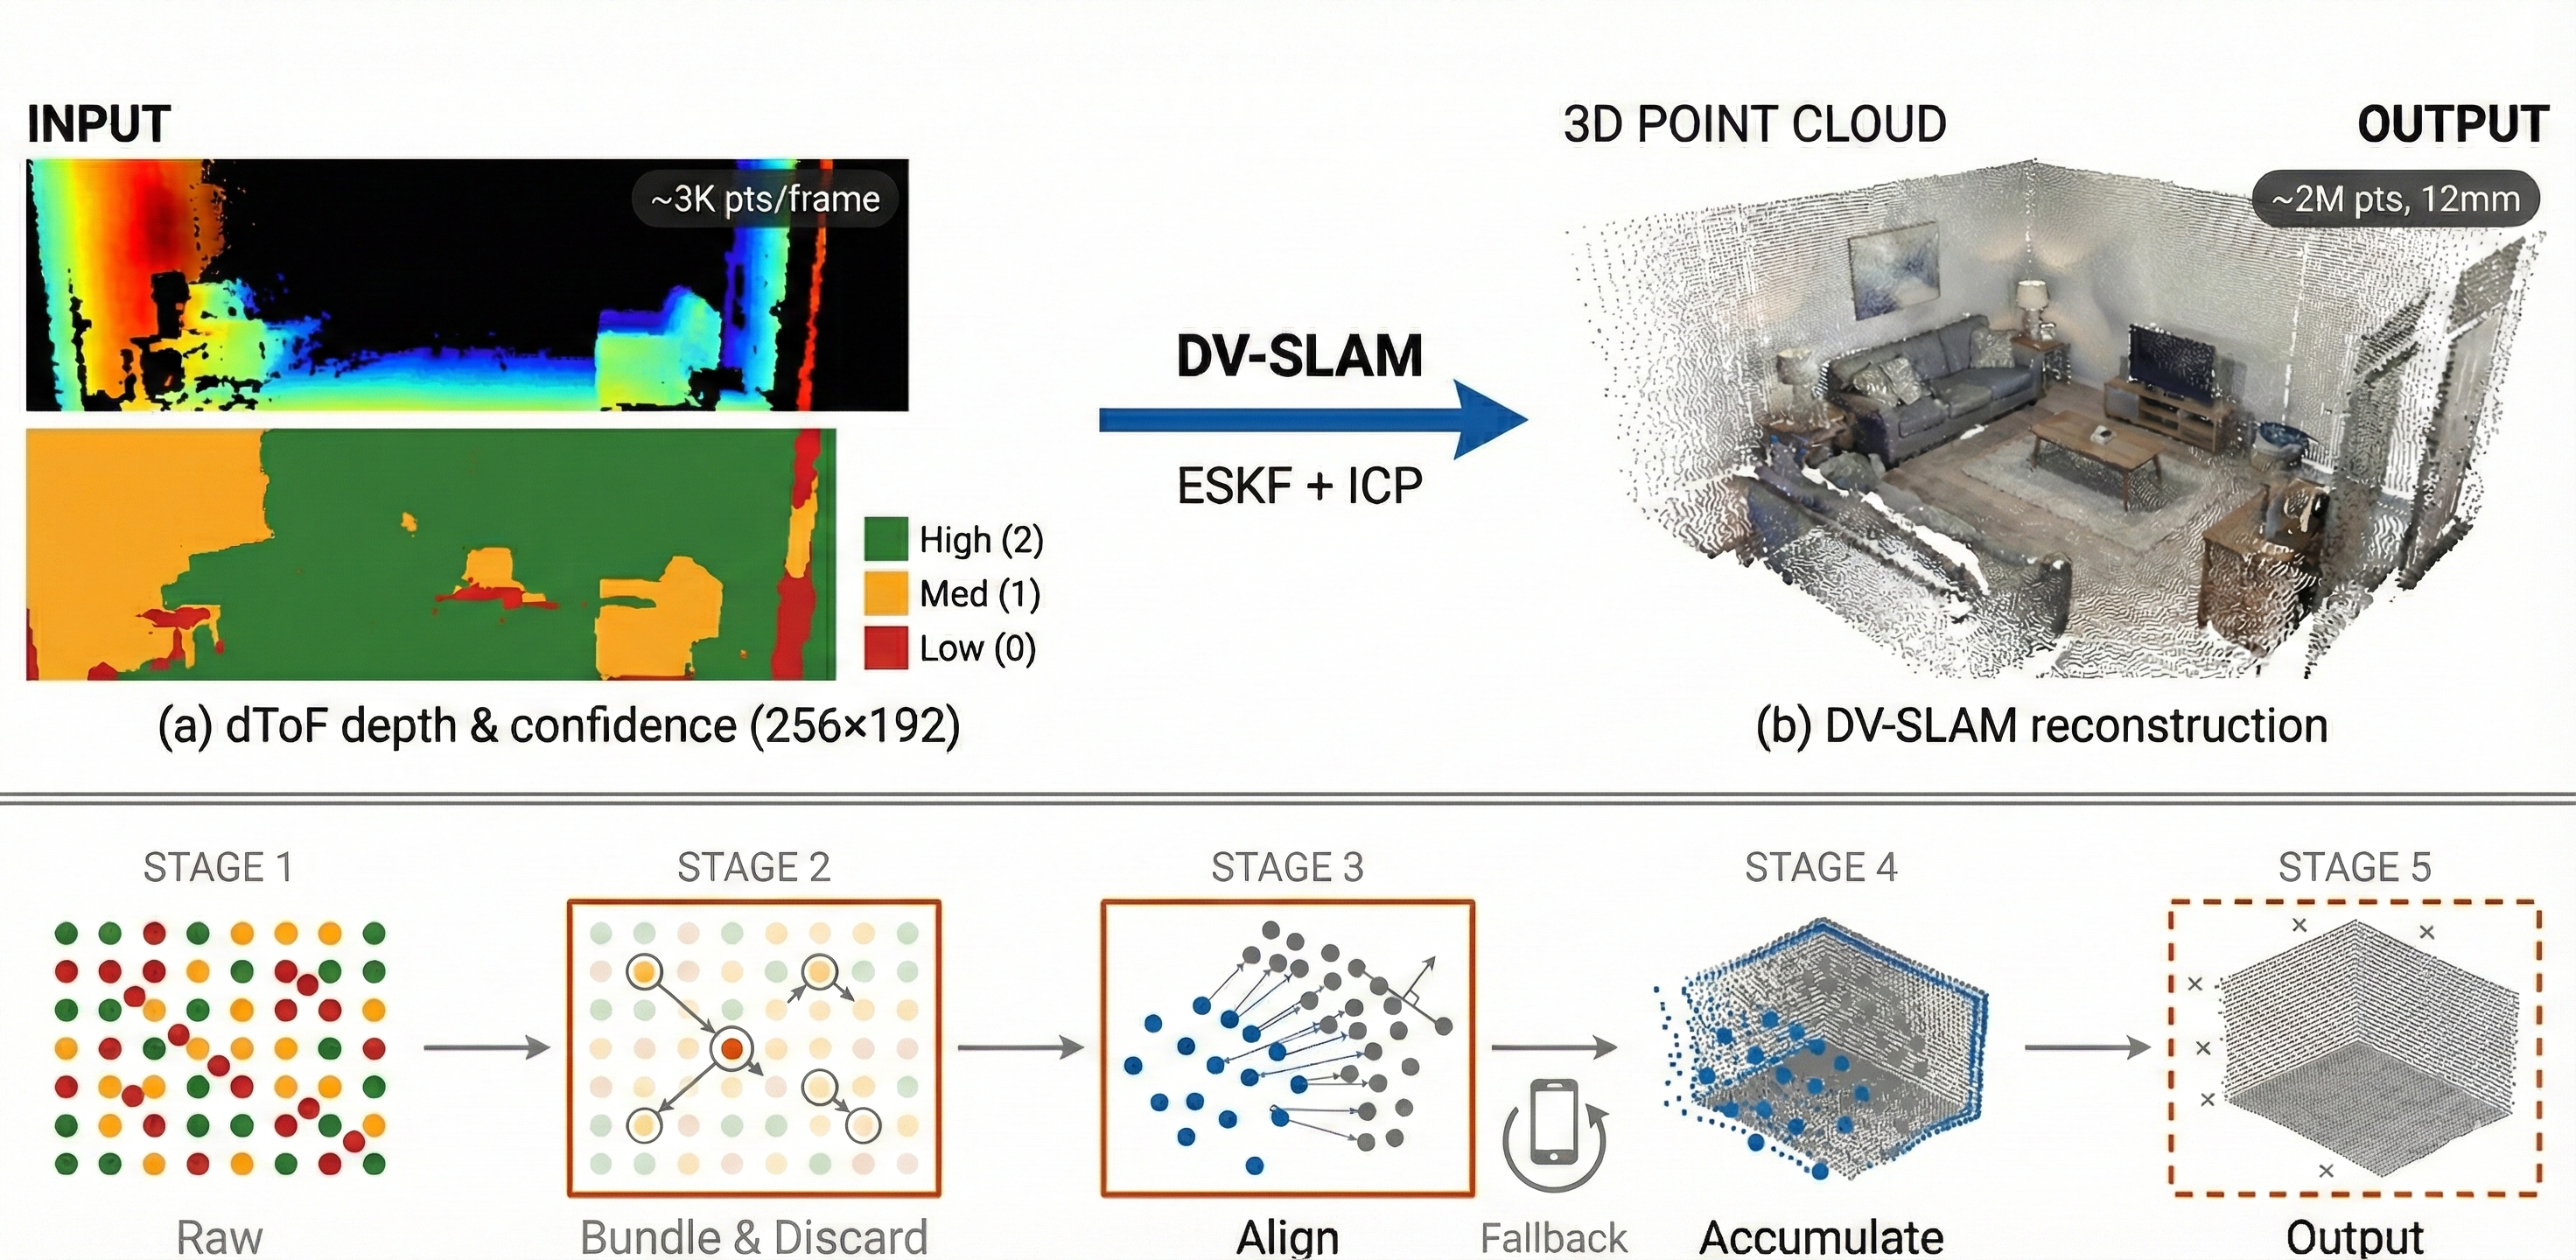
\includegraphics[width=\textwidth]{dvslam_fig1.png}
    \caption{Overview of DV-SLAM. (a)~Input: a single dToF frame produces a $256\!\times\!192$ depth map (${\sim}$3K points) with per-pixel confidence metadata (green = High, orange = Medium, red = Low). (b)~Output: the accumulated 3D point cloud (${\sim}$2M points at 12\,mm point spacing). Bottom: the five-stage pipeline. Orange borders indicate stages that exploit confidence metadata.}
    \label{fig:overview}
\end{figure*}

%% P2: dToF is a qualitatively different regime
Since 2020, hundreds of millions of smartphones have shipped with direct time-of-flight (dToF) LiDAR sensors. The dToF module on recent devices produces $256 \times 192$ depth maps at 30\,Hz. After quality filtering, only 200--500 points survive per frame, two orders of magnitude fewer than a typical mechanical LiDAR scan (Table~\ref{tab:sensor_comparison}). Quantization noise (1--5\,cm), multipath on reflective surfaces, and range-dependent degradation make dToF point quality highly non-uniform, unlike mechanical LiDARs where uniformity can be assumed.

\begin{table}[t]
    \centering
    \caption{Sensor comparison: consumer dToF vs.\ mechanical scanning LiDARs commonly used in LIO benchmarks. Consumer dToF column shows specifications of the Apple dToF module; Android dToF sensors have comparable resolution and range.}
    \label{tab:sensor_comparison}
    \setlength{\tabcolsep}{3.5pt}
    \begin{tabular}{lccc}
        \toprule
        Specification & Consumer dToF & VLP-16 & OS1-64 \\
        \midrule
        Principle & SPAD photon cnt. & ToF rotating & ToF rotating \\
        Resolution & $256 \times 192$ & 16 ch. & 64 ch. \\
        Points / frame & ${\sim}3$K eff. & ${\sim}30$K & ${\sim}131$K \\
        Range accuracy & 1--5\,cm & $\pm$3\,cm & $\pm$2.5\,cm \\
        Max range & ${\sim}5$\,m & 100\,m & 90\,m$^\dagger$ \\
        FOV (H$\times$V) & $60\times48^{\circ}$ & $360\times30^{\circ}$ & $360\times45^{\circ}$ \\
        Per-point quality & 3-level conf. & None & None \\
        Cost & Consumer phone & ${\sim}$\$4K$^\ddagger$ & ${\sim}$\$6K+ \\
        \bottomrule
        \multicolumn{4}{l}{\scriptsize $^\dagger$At 10\% reflectivity. $^\ddagger$Discontinued (Ouster acquisition).}
    \end{tabular}
\end{table}

%% P3: WHY existing LIO fails — three failure modes
This is not a scaled-down version of dense LIO; the sparse dToF regime is \emph{qualitatively different}. Dense-cloud systems (FAST-LIO2, DLIO, LIO-SAM~\cite{shan2020liosam}) do not gracefully degrade to $<$500-point data, because three failure modes, absent in the dense regime, become dominant:
\begin{itemize}
    \item[\textbf{F1.}] \textbf{ICP rank deficiency.} With $<$500 points spanning a narrow field of view ($60\times45^{\circ}$), the observation matrix frequently lacks sufficient geometric diversity for a well-conditioned 6-DoF update. Dense LIO with 10K+ points rarely encounters this issue.
    \item[\textbf{F2.}] \textbf{Single-point dominance.} When only 200--500 points contribute to the Kalman update, a single erroneous correspondence can corrupt the entire pose estimate. In dense LIO, one bad point among 10K is noise-floor.
    \item[\textbf{F3.}] \textbf{Blind downsampling destruction.} Standard voxel downsampling applied to 500 points can reduce them to $<$50, obliterating geometric constraint. Dense LIO can downsample 10K$\rightarrow$1K and still function.
\end{itemize}
The only currently available solutions on consumer devices are the manufacturer's closed-source visual-inertial odometry and open-source wrappers (e.g., RTAB-Map~\cite{labbe2019rtabmap}) that use it as a front-end. Both require camera input, offer no per-point quality control, and cannot operate when visual tracking degrades. Community attempts at camera-free LiDAR odometry on these devices have been unsuccessful due to the platform VIO's camera dependency~\cite{rtabmap_issue1026}. This leaves a gap: \emph{can tightly-coupled LIO operate robustly with fewer than 500 points per frame, and if so, what design principles are required?}

%% P4: dToF's unique asset — confidence metadata
dToF sensors provide a signal absent in mechanical LiDARs: \emph{per-pixel confidence metadata}. The dToF hardware classifies each depth pixel into three confidence levels (High, Medium, Low) based on photon-count signal-to-noise ratio. This metadata encodes measurement reliability not recoverable from the depth value alone. A 3-meter reading on a diffuse wall (High) and on glass (Low) produce identical depth values but vastly different accuracy.

%% P5: Thesis — confidence solves F1-F3
We show that this confidence metadata is the key to making LIO viable in the sparse regime, addressing all three failure modes.
F1 is mitigated by confidence gating, which rejects unreliable points early and ensures that surviving observations provide genuine geometric constraint.
F2 is addressed by confidence-weighted observation noise (Proposition~\ref{prop:fim}): matching weights to the true noise model yields the Best Linear Unbiased Estimator, minimizing the influence of low-quality points on the Kalman update. Proposition~\ref{prop:efficiency} quantifies the cost of ignoring this: uniform weighting inflates pose variance by ${\sim}$54\%.
F3 is solved by Confidence-Gated Downsampling (CGD), which reduces points based on quality rather than spatial proximity; Lemma~\ref{lem:cgd} guarantees that the information loss is bounded at $O(l_v^2 / r_{\min}^2)$.
Because only depth and inertial data enter the state estimation, the pipeline is entirely camera-free.

%% P6: Contributions
In this paper, we present DV-SLAM (Fig.~\ref{fig:overview}), a tightly-coupled LIO system designed from the ground up for sparse dToF data. Our contributions are:

\begin{enumerate}
    \item \textbf{Confidence-aware LIO for sparse dToF.} We show that per-pixel confidence metadata, a signal unique to dToF hardware and absent in mechanical LiDARs, is the key enabler for tightly-coupled LIO below 500 points per frame. Multi-level confidence exploitation, hard gating, quality-aware downsampling (CGD), and observation weighting, addresses the three failure modes (F1--F3) that prevent existing dense-cloud systems from operating in this regime. A Gauss--Markov analysis confirms that confidence-matched weighting is optimal; ignoring it inflates pose variance by ${\sim}$54\% (Proposition~\ref{prop:efficiency}).
    \item \textbf{Camera-free odometry on consumer hardware.} Because only depth and inertial measurements enter the state estimation, DV-SLAM performs 6-DoF pose estimation without camera images, the first demonstrated camera-free LIO on built-in mobile dToF sensors. The pipeline runs in real time (${\sim}$13\,ms/keyframe) on a mobile processor with a single Eigen dependency.
    \item \textbf{Sparse-regime characterization.} A point-count sweep (50--3{,}000 points) provides the first empirical characterization of the minimum viable observation count for stable LIO, quantifying the margin that confidence-aware processing provides over uniform treatment and identifying the collapse boundary.
\end{enumerate}
Source code will be released upon acceptance.

%% ============================================================
\section{Related Work}
\label{sec:related}
%% ============================================================

\subsection{LiDAR-Inertial Odometry}

FAST-LIO2~\cite{xu2022fastlio2} introduced IEKF with ikd-Tree, DLIO~\cite{chen2023dlio} simplified the pipeline via continuous-time correction, and LIO-SAM~\cite{shan2020liosam} added factor-graph optimization with loop closure. Visual-LiDAR-inertial extensions~\cite{zheng2024fastlivo2,lin2022r3live} and efficient variants~\cite{bai2022faster} have further broadened the field. KISS-ICP~\cite{vizzo2023kiss} showed that careful point-to-point ICP rivals more complex systems. All assume dense point clouds ($>$10K points/scan).

When applied to dToF data with $<$500 usable points, ICP degeneracy and bias accumulation become severe (Section~\ref{sec:experiments}).

\textbf{Sparse-observation odometry.} Sparse regimes arise outside dense LiDAR: automotive 4D radar produces ${\sim}$100--500 detections per scan~\cite{zhang2023radar,zhuang2023iriom,michalczyk2022rio}, and feature-based LIO methods operate on ${\sim}$100--500 extracted primitives from dense clouds. However, radar measurements have 10--50$\times$ coarser range resolution with continuous-valued SNR, and feature-based methods presuppose a dense input from which to extract. Consumer dToF differs in three respects: (i)~sparsity is inherent, not a design choice; (ii)~the sensor provides discrete per-pixel confidence metadata absent in radar or mechanical LiDAR; and (iii)~the noise structure is heteroscedastic with known class variances, admitting a closed-form optimal weighting (Proposition~\ref{prop:fim}). To our knowledge, no prior work addresses this specific combination.

\subsection{Mobile Depth Sensing and 3D Scanning}

ARKitScenes~\cite{baruch2021arkitscenes} provided the first large-scale RGB-D dataset from the iPad Pro dToF sensor, with FARO Focus S70 ground truth meshes. ScanNet++~\cite{yeshwanth2023scannetpp} extended this with high-fidelity DSLR and iPhone captures, complementing earlier benchmarks such as ScanNet~\cite{dai2017scannet} and TUM RGB-D~\cite{sturm2012benchmark}. Luetzenburg et al.~\cite{luetzenburg2021evaluation} evaluated iPad Pro LiDAR for geoscientific applications, reporting depth accuracy limitations. These works focus on depth quality or scene understanding; the question of building robust odometry \emph{natively} on sparse dToF has received limited attention.

Commercial scanning apps on dToF-equipped devices are uniformly closed-source and rely on the manufacturer's VIO for pose estimation; none disclose their odometry method or offer per-point quality control. RTAB-Map~\cite{labbe2019rtabmap} provides an open-source alternative on iOS, but explicitly uses the platform's visual-inertial odometry as its SLAM front-end, requiring camera input; community attempts at LiDAR-only operation have been unsuccessful due to this dependency~\cite{rtabmap_issue1026}. A recent preprint~\cite{liu2025livoxphone} runs Faster-LIO on an Android smartphone, but attaches an external Livox Mid-360 (${\sim}$200K points/scan, $360^{\circ}$ FoV) to the phone as a compute platform; this addresses mobile computation, not sensor sparsity. To our knowledge, no peer-reviewed open-source LIO system has been validated on built-in mobile dToF data with $<$500 points per frame, and no existing system, open or commercial, performs camera-free odometry on this hardware.

\subsection{Confidence and Quality-Aware SLAM}

Incorporating measurement uncertainty into SLAM has been widely studied. Kerl et al.~\cite{kerl2013robust} introduced robust weighting for RGB-D odometry based on $t$-distribution residual models. Nguyen et al.~\cite{nguyen2012modeling} characterized Kinect depth noise as a function of distance and incidence angle. Tateno et al.~\cite{tateno2017cnnslam} predicted per-pixel depth confidence from monocular CNNs for dense SLAM, and Czarnowski et al.~\cite{czarnowski2020deepfactors} incorporated learned depth uncertainty into factor graphs. In the LiDAR domain, per-point quality has received less attention: KISS-ICP~\cite{vizzo2023kiss} uses adaptive thresholding but no explicit quality indicators.

The dToF confidence signal is distinct from these approaches: it is a discrete three-level classification derived from photon-count signal-to-noise ratio, encoding measurement reliability inaccessible from the depth value alone. To our knowledge, DV-SLAM is the first LIO system to exploit this metadata across the full pipeline.

Table~\ref{tab:pipeline_comparison} summarizes the structural differences between DV-SLAM and representative LIO systems.

\begin{table}[t]
    \centering
    \caption{Pipeline comparison with representative LIO systems~\cite{xu2022fastlio2,chen2023dlio,shan2020liosam}. DV-SLAM operates on 10--500$\times$ fewer points and is the only system exploiting per-point quality metadata.}
    \label{tab:pipeline_comparison}
    \setlength{\tabcolsep}{2.5pt}
    \footnotesize
    \begin{tabular}{lcccc}
        \toprule
        Feature & FAST-LIO2 & DLIO & LIO-SAM & \textbf{Ours} \\
        \midrule
        Target sensor & Mech. & Mech. & Mech. & dToF \\
        Filter / optim. & IEKF$^\dagger$ & GICP & Factor gr. & IEKF$^\dagger$ \\
        Pts. / frame & 10--100K+ & 10--100K+ & 10--100K+ & 200--500 \\
        Quality weight & \ding{55} & \ding{55} & \ding{55} & 3-level \\
        Adaptive reduction & Voxel & Voxel & Voxel & Dens.+conf. \\
        Loop closure & \ding{55} & \ding{55} & \ding{51} & \ding{55} \\
        Dependencies & ${\sim}50$MB+ & ${\sim}30$MB+ & ${\sim}80$MB+ & ${\sim}3$MB \\
        Open source & \ding{51} & \ding{51} & \ding{51} & \ding{51} \\
        \bottomrule
        \multicolumn{5}{l}{\scriptsize $^\dagger$Both use iterated ESKF on $SO(3)$; the key difference is}\\
        \multicolumn{5}{l}{\scriptsize \phantom{$^\dagger$}confidence-weighted observations (row 4).}
    \end{tabular}
\end{table}

%% ============================================================
\section{Method}
\label{sec:method}
%% ============================================================

DV-SLAM requires three sensor inputs: (i)~a sparse depth map with per-pixel confidence metadata, (ii)~6-axis IMU measurements at $\geq$100\,Hz, and (iii)~camera intrinsics for depth back-projection. No camera images enter the state estimation; RGB is used only for optional point cloud colorization.

\subsection{Depth Back-Projection and Confidence Extraction}
\label{sec:backproj}

We define the world frame $\mathcal{W}$ (gravity along $-y$), the IMU body frame $\mathcal{B}$, and the camera frame $\mathcal{C}$ ($y$-down, $z$-forward). Points are transformed between camera and world conventions via a coordinate reflection $\mathbf{M} = \text{diag}(1,-1,-1)$ that converts the $y$-down/$z$-forward camera convention to the $y$-up world frame. We approximate the camera-IMU extrinsic as identity ($\mathbf{T}_{\mathcal{C}\mathcal{B}} \approx \mathbf{I}$); on typical dToF-equipped devices the lever arm is 5--10\,mm, introducing ${\sim}$1\,cm error at typical angular velocities, within the dToF noise floor (Section~\ref{sec:limitations}).

Each captured frame provides a depth map $\mathbf{D} \in \mathbb{R}^{256 \times 192}$ and a confidence map $\mathbf{C} \in \{0, 1, 2\}^{256 \times 192}$. Since camera intrinsics $\mathbf{K}$ are provided at capture resolution ($1920 \times 1440$), we scale to depth resolution: $f'_x = f_x \cdot W_{\text{depth}} / W_{\text{cam}}$. Unlike mechanical scanning LiDARs, the dToF sensor captures the entire depth map simultaneously (flash operation)~\cite{luetzenburg2021evaluation}, eliminating the need for intra-frame motion compensation (de-skewing). We back-project at a stride of 4 pixels, yielding ${\sim}$3{,}000 candidate points $\{\mathbf{p}_i^{\mathcal{C}}, c_i\}$, where $c_i \in \{0,1,2\}$ is the confidence level.

\textbf{Hard gate.} Points with $c_i = 0$ (Low) are discarded. This removes measurements from transparent surfaces, specular reflections, and out-of-range regions where the photon-count SNR is insufficient.

\begin{table}[t]
    \centering
    \caption{dToF confidence levels: empirical characteristics measured on a $256 \times 192$ dToF sensor (see Section~\ref{sec:datasets} for hardware details).}
    \label{tab:confidence_levels}
    \setlength{\tabcolsep}{3pt}
    \footnotesize
    \begin{tabular}{lcccl}
        \toprule
        Level & Value & Depth error & Proportion & Pipeline action \\
        \midrule
        High & 2 & ${\sim}1$\,cm & 40--50\% & Full weight ($w = 1.0$) \\
        Medium & 1 & ${\sim}2$--3\,cm & 30--40\% & Reduced ($w = 0.5$) \\
        Low & 0 & ${\sim}3$--5+\,cm & 10--20\% & Hard reject \\
        \bottomrule
    \end{tabular}
\end{table}

\subsection{Confidence-Gated Downsampling}
\label{sec:cgd}

After the hard gate, the remaining ${\sim}$2{,}400 points undergo adaptive reduction that jointly considers spatial density and measurement confidence.

\textbf{Step 1: Spatial hashing.} Points are discretized into voxels of size $l_v$ (Table~\ref{tab:parameters}) via hash map $\mathcal{V}: \mathbb{Z}^3 \rightarrow \{\mathbf{p}_i, c_i\}$.

\textbf{Step 2: Density filtering.} Voxels with fewer than $\tau_d$ points are discarded. Isolated points in sparse voxels are disproportionately likely to be noise.

\textbf{Step 3: Confidence filtering.} Voxels whose mean confidence falls below a threshold are discarded. This removes spatially coherent but unreliable regions (e.g., a cluster of Medium-confidence points on a distant reflective surface).

\textbf{Step 4: Centroid extraction.} Each surviving voxel emits a single representative point (centroid), tagged with the mean confidence of the voxel.

This cascade reduces ${\sim}$2{,}400 post-gate points to ${\sim}$200--500 high-quality correspondences while preserving geometric diversity across the field of view. The key distinction from standard voxel downsampling is that density \emph{and} confidence jointly determine survival: a dense cluster of Medium-confidence points on glass is discarded, while sparse but High-confidence points on a diffuse wall are retained. An alternative is to use all ${\sim}$2{,}400 points with confidence weighting but no reduction; we include this configuration in the ablation (Table~\ref{tab:ablation}) to verify that quality-aware reduction outperforms brute-force inclusion, as noisy correspondences degrade local plane fitting even when downweighted.

\textbf{Information preservation.}

\begin{lemma}[Centroid FIM loss]
\label{lem:cgd}
Let a voxel of size $l_v$ contain $k$ co-planar points on a surface with minimum curvature radius $r_{\min}$. Replacing the $k$ points with a single centroid incurs a relative point-to-plane Fisher Information loss bounded by $O(l_v^2 / r_{\min}^2)$.
\end{lemma}

\textit{Proof sketch.} The angular deviation between per-point normals and the centroid normal within a voxel of size $l_v$ is bounded by $l_v/r_{\min}$; squaring gives the stated bound. At edges where the co-planar assumption breaks, the density filter ($\tau_d$) retains voxels only when sufficient points constrain both normals. \hfill$\square$

At $l_v = 0.1$\,m and $r_{\min} \geq 0.5$\,m (typical indoor walls), the bound gives $\leq 4$\% information loss per voxel. The 80--90\% point reduction in CGD thus comes almost entirely from removing redundant co-planar observations, not from discarding geometric constraint. An ablation row (Table~\ref{tab:ablation}, ``All ${\sim}$2400 pts'') verifies this empirically.

\subsection{IEKF State Estimation}
\label{sec:fisher}

We adopt the IEKF formulation of FAST-LIO2~\cite{xu2021fastlio,xu2022fastlio2} on the 18D state $\mathbf{x}_k = [\mathbf{R}_k,\,\mathbf{p}_k,\,\mathbf{v}_k,\,\mathbf{b}_{g,k},\,\mathbf{b}_{a,k},\,\mathbf{g}]$ ($\delta\mathbf{x} \in \mathbb{R}^{18}$); the standard ESKF derivation follows~\cite{sola2017quaternion,barfoot2017state}. Three modifications address the sparse regime. First, IMU propagation uses midpoint integration ($\mathbf{R}_{\text{mid}} = \mathbf{R}_k \cdot \text{Exp}(\boldsymbol{\omega}\,\Delta t / 2)$), eliminating first-order angular-velocity bias under handheld rotation. Second, we set $\mathbf{Q}_p = \sigma_a^2 \Delta t^3/4\;\mathbf{I}_3$ (conservative) rather than the exact $\sigma_a^2 \Delta t^5/20$, biasing the Kalman gain toward the confidence-weighted measurements when only 200--500 observations constrain the update. The third and most important modification is the confidence-weighted observation noise $\mathbf{R}_{\text{obs}}$ (Section~\ref{sec:icp}), motivated by the analysis below.

Before detailing the ICP implementation, we quantify the cost of ignoring dToF confidence metadata.

\begin{proposition}[dToF-optimal weighting]
\label{prop:fim}
Consider $N$ point-to-plane observations from a dToF sensor, partitioned into $N_H$ High-confidence measurements with variance $\sigma_H^2$ and $N_M$ Medium-confidence measurements with variance $\sigma_M^2$. The confidence-matched weighting $w_i = \sigma_H^2 / \sigma_{c_i}^2$ (i.e., $\mathbf{W} = \mathbf{R}_{\text{true}}^{-1}$) yields the Best Linear Unbiased Estimator (BLUE) for the 6-DoF pose. The corresponding Fisher Information is
\begin{equation}
    I_{\text{opt}} \propto \frac{N_H}{\sigma_H^2} + \frac{N_M}{\sigma_M^2}
    \label{eq:fim_opt}
\end{equation}
whereas uniform weighting ($w_i = 1$) achieves only
\begin{equation}
    I_{\text{uni}} \propto \frac{N^2}{N_H \sigma_H^2 + N_M \sigma_M^2}
    \label{eq:fim_uni}
\end{equation}
with $I_{\text{opt}} \geq I_{\text{uni}}$ always, equality holding only when $\sigma_H = \sigma_M$.
\end{proposition}

\textit{Proof.} Direct application of the Gauss--Markov theorem~\cite{barfoot2017state}: setting $\mathbf{W} = \mathbf{R}_{\text{true}}^{-1}$ minimizes the estimation covariance; any other diagonal $\mathbf{W}'$ inflates the trace via the Cauchy--Schwarz inequality. \hfill$\square$

\begin{proposition}[Variance inflation ratio]
\label{prop:efficiency}
Under isotropic observation geometry, the ratio of pose variance under uniform weighting to that under confidence-matched weighting is:
\begin{equation}
    \eta = 1 + \frac{N_H N_M (\sigma_M^2 - \sigma_H^2)^2}{N^2\,\sigma_H^2\,\sigma_M^2}
    \label{eq:efficiency}
\end{equation}
For the measured dToF noise profile ($N_H/N = 0.6$, $\sigma_H = 1$\,cm, $\sigma_M = 2$\,cm; Table~\ref{tab:confidence_levels}), $\eta \approx 1.54$: uniform weighting inflates pose variance by ${\sim}$54\%.
\end{proposition}

\textit{Proof.} Direct algebraic expansion of $I_{\text{opt}} / I_{\text{uni}}$ from Proposition~\ref{prop:fim}. \hfill$\square$

\subsection{Point-to-Plane ICP via IEKF}
\label{sec:icp}

Propositions~\ref{prop:fim}--\ref{prop:efficiency} establish that confidence-matched weighting is optimal; we now detail how this weighting enters the IEKF update. For each keyframe, we perform point-to-plane ICP~\cite{pomerleau2015review} within the IEKF framework (up to 3 iterations, early termination at $\|\delta\mathbf{x}\| < 10^{-6}$).

\textbf{Correspondence search.} Each point $\mathbf{p}_i^{\mathcal{C}}$ is transformed to the world frame and queried against the global map. $K$ nearest neighbors are retrieved, and a local plane is fitted via SVD. A planarity check $\lambda_0 / \lambda_1 < \tau_{\text{plan}}$ (Table~\ref{tab:parameters}) rejects non-planar correspondences, where a low ratio confirms a locally planar distribution. If fewer than $N_{\min} = 10$ valid correspondences survive, the IEKF update is skipped and the filter relies on IMU-only propagation, preventing poorly constrained pose updates.

\textbf{Observation model.} For point $\mathbf{p}_i^{\mathcal{C}}$ with correspondence plane $(\mathbf{n}_j, \bar{\mathbf{q}}_j)$:
\begin{equation}
    r_i = \mathbf{n}_j^\top \left( \mathbf{R}\,\mathbf{p}_i^{\mathcal{C}} + \mathbf{p} - \bar{\mathbf{q}}_j \right)
    \label{eq:residual}
\end{equation}
\begin{equation}
    \mathbf{H}_i = \left[ -\mathbf{n}_j^\top \mathbf{R} [\mathbf{p}_i^{\mathcal{C}}]_\times,\;\; \mathbf{n}_j^\top,\;\; \mathbf{0}_{1 \times 12} \right]
    \label{eq:jacobian}
\end{equation}

\textbf{Confidence-weighted robust kernel.} Each residual is weighted by $w_i = w_i^{\text{conf}} \cdot w_i^{\text{TLS}}$, where:
\begin{equation}
    w_i^{\text{conf}} = \frac{\sigma_H^2}{\sigma_{c_i}^2}, \qquad
    w_i^{\text{TLS}} = \begin{cases}
        1 & \text{if } |r_i| \leq \tau_{\text{TLS}} \\
        0 & \text{otherwise}
    \end{cases}
    \label{eq:weight}
\end{equation}
The noise-model-derived optimal is $w_M = 0.25$, but intra-class variance in Medium-confidence measurements motivates $w_M = 0.5$ as a robust compromise; the ablation (Table~\ref{tab:ablation}) confirms stability across $[0.25, 0.75]$ and meaningful degradation only at $w_M = 1.0$ (uniform). The TLS threshold is set to ${\sim}3\times$ the dToF noise floor.

\textbf{Kalman update.} The weights enter through the observation noise covariance:
\begin{equation}
    \mathbf{R}_{\text{obs}}(i,i) = \frac{\sigma_{\text{base}}^2}{\max(w_i,\;\epsilon)}, \quad \epsilon = 0.01
    \label{eq:Robs}
\end{equation}
where $\sigma_{\text{base}}^2 = 10^{-4}$\,m$^2$ ($\sigma_{\text{base}} = 1$\,cm). The Kalman gain is computed via LDLT decomposition of $\mathbf{S} = \mathbf{H}\mathbf{P}\mathbf{H}^\top + \mathbf{R}_{\text{obs}}$, and the covariance is updated using the Joseph form for numerical stability. Rotation is injected via right multiplication: $\mathbf{R} \leftarrow \mathbf{R} \cdot \text{Exp}(\delta\hat{\boldsymbol{\theta}})$.

\subsection{Keyframe Selection and Divergence Guard}
\label{sec:divergence}

A new keyframe is declared when $\|\mathbf{p}_k - \mathbf{p}_{\text{last}}\| \geq \tau_p$ or $\angle(\mathbf{R}_k, \mathbf{R}_{\text{last}}) \geq \tau_r$. Non-keyframes use IMU-only propagation.

The ESKF may diverge due to poor ICP correspondences. The filter monitors the trace of the pose covariance $\text{tr}(\mathbf{P}_{1:6,1:6})$. When it exceeds $\tau_{\text{cov}}$ (Table~\ref{tab:parameters}), the current ICP update is discarded (not the filter state), and the filter continues with IMU-only propagation. The covariance grows monotonically during IMU-only intervals; the next keyframe's ICP update, if successful ($\geq N_{\min}$ correspondences with residual below $\tau_{\text{TLS}}$), constrains the grown covariance back to acceptable levels.

\subsection{Map Management}
\label{sec:map}

Refined points are inserted into a spatial hash map (voxel size 0.1\,m). Each voxel stores up to 20 points with precomputed centroid and covariance for nearest-neighbor queries. Upon export, surface thinning resolves double-wall artifacts from repeated observations.

Table~\ref{tab:parameters} lists the DV-SLAM-specific parameters; all values remained fixed across experiments.

\begin{table}[t]
    \centering
    \caption{DV-SLAM parameters. All values are fixed across experiments.}
    \label{tab:parameters}
    \setlength{\tabcolsep}{3pt}
    \footnotesize
    \begin{tabular}{llrl}
        \toprule
        Stage & Parameter & Value & Rationale \\
        \midrule
        \multicolumn{4}{l}{\textit{Conf.-Gated Downsamp. (\S\ref{sec:cgd})}} \\
        & Voxel size $l_v$ & 0.1\,m & Spatial binning \\
        & Min.\ density $\tau_d$ & 5\,pts & Noise suppression \\
        & Mean conf.\ threshold & 1.5 & Majority High \\
        \midrule
        \multicolumn{4}{l}{\textit{Keyframe / Div.\ Guard (\S\ref{sec:divergence})}} \\
        & Transl.\ threshold $\tau_p$ & 5\,cm & Sufficient baseline \\
        & Rot.\ threshold $\tau_r$ & $2^{\circ}$ & New geometry \\
        & Cov.\ trace $\tau_{\text{cov}}$ & 1.0\,m$^2$ & Divergence detect \\
        \midrule
        \multicolumn{4}{l}{\textit{ICP / IEKF (\S\ref{sec:icp})}} \\
        & Nearest neighbors $K$ & 5 & Plane fitting \\
        & Planarity $\lambda_0/\lambda_1$ & $<0.3$ & Planar check \\
        & Min.\ correspondences $N_{\min}$ & 10 & Rank safety \\
        & TLS threshold $\tau_{\text{TLS}}$ & 10\,cm & $3\times$ dToF noise \\
        & Base noise $\sigma_{\text{base}}$ & 1\,cm & Eq.~\eqref{eq:Robs} \\
        & $w_M$ (Medium weight) & 0.5 & Sec.~\ref{sec:icp} \\
        \bottomrule
        \multicolumn{4}{l}{\scriptsize IMU noise parameters follow manufacturer specifications.}
    \end{tabular}
\end{table}

\textbf{Hardware.} All experiments run on an iPhone 14 Pro (Apple A16 Bionic, single-thread, 6\,GB RAM, iOS 17). The full ESKF+ICP update completes in ${\sim}$13\,ms per keyframe without GPU acceleration. The entire codebase depends only on Eigen headers (${\sim}$3\,MB).

%% ============================================================
\section{Experiments}
\label{sec:experiments}
%% ============================================================

We evaluate DV-SLAM against three questions: (1)~Can tightly-coupled LIO operate with $<$500 points per frame? (2)~Is confidence-aware weighting essential or merely helpful? (3)~At what point count does LIO collapse, and can confidence-aware processing close the quality gap between a consumer dToF sensor and dedicated scanning hardware?

\subsection{Datasets and Ground Truth}
\label{sec:datasets}

\textbf{Self-collected sequences.}
We collect five sequences on an iPhone~14~Pro using Stray Scanner, logging raw IMU (100\,Hz), dToF depth and confidence (30\,Hz), and concurrent ARKit poses for reference. Each trajectory forms a closed loop (start $=$ end). We report two trajectory metrics: (1)~end-to-end loop closure drift as a percentage of trajectory length, and (2)~ATE RMSE against concurrent ARKit poses (SE(3)-aligned via \texttt{evo}) as a continuous trajectory reference. Sequences span five conditions:

\begin{table}[t]
    \centering
    \caption{Self-collected evaluation sequences.}
    \label{tab:sequences}
    \setlength{\tabcolsep}{4pt}
    \begin{tabular}{clcc}
        \toprule
        Seq. & Condition & Length & Purpose \\
        \midrule
        S1 & Normal indoor (room) & ${\sim}$20\,m & Baseline \\
        S2 & Long corridor & ${\sim}$30\,m & Drift \\
        S3 & Fast rotation ($>$2\,rad/s) & ${\sim}$15\,m & IMU stress \\
        S4 & Glass / reflective & ${\sim}$15\,m & Confidence effect \\
        S5 & Bright outdoor & ${\sim}$20\,m & dToF limit \\
        \bottomrule
    \end{tabular}
\end{table}

\textbf{ARKitScenes~\cite{baruch2021arkitscenes}.}
We use the high-resolution subset with FARO Focus S70 ground truth meshes for map quality evaluation (Accuracy, Completeness, F-score). Since ARKitScenes does not include raw IMU, this track evaluates the confidence-gated reconstruction only (depth + confidence + external poses).

\textbf{Dense reference maps (Livox Mid-70).}
For sequences S1, S2, and S4, we acquire independent dense reference point clouds using a Livox Mid-70 solid-state LiDAR (non-repetitive scanning, $\pm$2\,cm accuracy at indoor range), processed with FAST-LIO2 to produce dense maps ($>$1M points). These provide a second, fully independent ground truth for map quality evaluation alongside the FARO meshes in ARKitScenes.

\textbf{dToF noise characterization.}
We measure per-confidence depth noise by recording 100 static frames at each of five distances (0.5, 1, 2, 3, 4\,m) against a flat wall. Plane fitting residuals yield $\sigma(d, c)$ for each confidence level and distance, grounding the noise model in Table~\ref{tab:confidence_levels} and the efficiency ratio $\eta$ in Proposition~\ref{prop:efficiency}. \todo{Insert noise characterization figure.}

\subsection{Baselines}
\label{sec:baselines}

\begin{enumerate}
    \item \textbf{ARKit (platform VIO).} Apple's visual-inertial odometry and reconstruction pipeline, the only currently available closed-source solution on this hardware. Requires active camera input.
    \item \textbf{RTAB-Map}~\cite{labbe2019rtabmap}: Open-source graph-based SLAM using ARKit VIO as the odometry front-end and dToF depth for loop closure refinement. This baseline uses both camera and dToF, isolating the value of camera-free operation.
    \item \textbf{Naive ICP}: DV-SLAM pipeline with uniform weights ($w_i^{\text{conf}} = 1.0$) and no CGD quality gate. Isolates the benefit of confidence-aware processing.
    \item \textbf{DV-SLAM (full)}: Default configuration with confidence gating and $w_M = 0.5$.
\end{enumerate}
Existing dense-cloud LIO systems (FAST-LIO2, DLIO, LIO-SAM) assume $>$10K points/scan. To contextualize the sparse regime, we replay S1 through FAST-LIO2~\cite{xu2022fastlio2} via a custom depth-to-\texttt{PointCloud2} bridge (ROS Noetic); \todo{report result: drift / degraded accuracy / divergence, confirming that dense-cloud LIO does not gracefully degrade to this regime}.

\subsection{Main Results}
\label{sec:results}

\begin{table}[t]
    \centering
    \caption{Main comparison on self-collected sequences (mean over S1--S5). Drift $=$ loop closure error / trajectory length. ATE $=$ RMSE vs.\ ARKit poses after SE(3) alignment.}
    \label{tab:main_comparison}
    \begin{tabular}{lccccc}
        \toprule
        Method & Cam. & Drift [\%] $\downarrow$ & ATE [cm] $\downarrow$ & Acc.\ [cm] $\downarrow$ & F-score $\uparrow$ \\
        \midrule
        ARKit (platform) & \checkmark & --- & (ref.) & \todo{--} & \todo{--} \\
        RTAB-Map & \checkmark & \todo{--} & \todo{--} & \todo{--} & \todo{--} \\
        Naive ICP ($w = 1$) & $\times$ & \todo{--} & \todo{--} & \todo{--} & \todo{--} \\
        \textbf{DV-SLAM (ours)} & $\times$ & \todo{--} & \todo{--} & \todo{--} & \todo{--} \\
        \bottomrule
    \end{tabular}
\end{table}

On two ARKitScenes sequences with FARO S70 ground truth, the confidence-gated reconstruction achieves \todo{X}\,cm accuracy and \todo{Y} F-score, consistent with the self-collected results.

\subsection{Ablation Study}
\label{sec:ablation}

\begin{table}[t]
    \centering
    \caption{Ablation on S1 (normal indoor). Each row modifies one aspect of the full pipeline.}
    \label{tab:ablation}
    \begin{tabular}{lcccc}
        \toprule
        Configuration & Drift [\%] & ATE [cm] & Acc.\ [cm] & F-score \\
        \midrule
        Full DV-SLAM & \todo{--} & \todo{--} & \todo{--} & \todo{--} \\
        $-$ Confidence ($w_i = 1$) & \todo{--} & \todo{--} & \todo{--} & \todo{--} \\
        $-$ CGD $\rightarrow$ uniform voxel DS & \todo{--} & \todo{--} & \todo{--} & \todo{--} \\
        ${\sim}$100 pts (stride 12) & \todo{--} & \todo{--} & \todo{--} & \todo{--} \\
        All ${\sim}$2400 pts, no CGD & \todo{--} & \todo{--} & \todo{--} & \todo{--} \\
        \bottomrule
    \end{tabular}
\end{table}

Row~2 directly tests the prediction of Proposition~\ref{prop:efficiency}: removing confidence weighting should inflate drift by a margin consistent with $\eta \approx 1.54$. Row~3 tests CGD versus standard voxel downsampling. Row~4 probes the collapse boundary. Row~5 verifies that CGD's quality-aware reduction outperforms brute-force inclusion of all points (Section~\ref{sec:cgd}).

\textbf{Point-count sweep.} On S1, we vary the back-projection stride $\{1, 4, 8, 12, 16\}$ yielding ${\sim}\{3000, 500, 200, 100, 50\}$ points per frame, each with confidence ON/OFF. This identifies the collapse threshold and quantifies the margin that confidence weighting provides. \todo{Insert point-count sweep figure.}

\textbf{Runtime.} On the A16 Bionic (single-thread, no GPU), the full pipeline completes in ${\sim}$13\,ms per keyframe: ESKF prediction ${\sim}$2\,ms, CGD ${\sim}$3\,ms, ICP update ${\sim}$8\,ms, comfortably exceeding the 10\,Hz keyframe rate. Peak memory is \todo{XX}\,MB.

\begin{figure*}[t]
    \centering
    \todo{Insert 4-column qualitative comparison: [ARKit recon] | [RTAB-Map] | [DV-SLAM no conf] | [DV-SLAM full]}
    \caption{Qualitative map comparison on \todo{sequence}. From left to right: ARKit reconstruction, RTAB-Map (camera + dToF), DV-SLAM without confidence weighting, DV-SLAM with full confidence pipeline. Note \todo{specific visual differences}.}
    \label{fig:qualitative}
\end{figure*}

%% ============================================================
\section{Discussion}
\label{sec:discussion}
%% ============================================================

\subsection{Generalization Beyond Apple dToF}

The confidence-aware pipeline is not Apple-specific. The core requirement is a per-pixel quality signal correlated with depth accuracy; Android ToF sensors (e.g., Samsung Galaxy S20+ with Sony DepthVision) expose analogous confidence or amplitude channels. Adapting DV-SLAM to these platforms requires only remapping the confidence classification to the weight function in Eq.~\eqref{eq:weight}. More broadly, any heteroscedastic depth sensor with known class structure, such as learned monocular uncertainty, event-camera confidence, or next-generation LiDAR SNR, benefits from matched weighting, and the penalty for ignoring it scales with the variance ratio (Eq.~\eqref{eq:efficiency}).

\subsection{Camera-Free Spatial Perception}

Current consumer 3D perception relies exclusively on visual-inertial odometry~\cite{campos2021orbslam3,qin2018vins} (VIO), which requires camera images as the primary sensing modality. DV-SLAM demonstrates that camera-free LiDAR-inertial odometry is viable on existing consumer hardware: the 6-DoF pose is estimated entirely from dToF depth and IMU, with RGB used only for optional point cloud colorization.
This enables privacy-preserving scanning in sensitive spaces (hospitals, residences) where no camera images need be stored, and provides a fallback when VIO fails (hand covering the camera, extreme lighting transitions).

\subsection{Limitations}
\label{sec:limitations}

\textbf{Camera-IMU extrinsic.} The identity approximation for $\mathbf{T}_{\mathcal{C}\mathcal{B}}$ introduces systematic error scaling with angular velocity. For aggressive motion ($>$3\,rad/s), the lever-arm error may exceed the dToF noise floor.

\textbf{Observability.} A formal rank analysis of the observability Gramian is beyond the scope of this paper. Empirically, the filter requires rotational motion and at least two non-parallel surfaces for stable convergence; the Divergence Guard provides practical detection of degenerate configurations. We leave formal observability analysis for future work.

\textbf{No loop closure.} Drift accumulates over long trajectories. Surface Thinning mitigates double-wall artifacts but does not correct the underlying trajectory error.

\textbf{No external pose fallback.} An external pose source can optionally assist divergence recovery; this extension is left for future work.

%% ============================================================
\section{Conclusion}
\label{sec:conclusion}
%% ============================================================

DV-SLAM demonstrates that tightly-coupled LIO is viable with fewer than 500 points per frame when confidence metadata guides every processing stage, from point selection through state estimation. The pipeline runs in real time on a mobile processor, requiring only Eigen and no camera input. Our results on \todo{datasets} show that confidence-aware processing is necessary to close the gap between consumer dToF sensors and reliable 3D scanning, and the point-count sweep identifies the boundary at which sparse-regime LIO remains viable.

\section*{Acknowledgment}
The authors thank \todo{acknowledgments}.

%% ============================================================
%% References
%% ============================================================
\begin{thebibliography}{25}

\bibitem{xu2022fastlio2}
W.~Xu, Y.~Cai, D.~He, J.~Lin, and F.~Zhang, ``FAST-LIO2: Fast direct LiDAR-inertial odometry,'' \textit{IEEE Trans. Robot.}, vol.~38, no.~4, pp.~2053--2073, 2022.

\bibitem{xu2021fastlio}
W.~Xu and F.~Zhang, ``FAST-LIO: A fast, robust LiDAR-inertial odometry package by tightly-coupled iterated Kalman filter,'' \textit{IEEE Robot. Autom. Lett.}, vol.~6, no.~2, pp.~3317--3324, 2021.

\bibitem{chen2023dlio}
K.~Chen, R.~Nemiroff, and B.~T.~Lopez, ``Direct LiDAR-inertial odometry: Lightweight LIO with continuous-time motion correction,'' \textit{IEEE Robot. Autom. Lett.}, vol.~8, no.~8, pp.~4828--4835, 2023.

\bibitem{shan2020liosam}
T.~Shan, B.~Englot, D.~Meyers, W.~Wang, C.~Ratti, and D.~Rus, ``LIO-SAM: Tightly-coupled lidar inertial odometry via smoothing and mapping,'' in \textit{Proc. IEEE/RSJ Int. Conf. Intell. Robots Syst. (IROS)}, 2020, pp.~5135--5142.

\bibitem{baruch2021arkitscenes}
G.~Baruch \textit{et al.}, ``ARKitScenes: A diverse real-world dataset for 3D indoor scene understanding using mobile RGB-D data,'' in \textit{Proc. Neural Inf. Process. Syst. (NeurIPS) Datasets and Benchmarks Track}, 2021.

\bibitem{yeshwanth2023scannetpp}
C.~Yeshwanth, Y.-C.~Liu, M.~Nie{\ss}ner, and A.~Dai, ``ScanNet++: A high-fidelity dataset of 3D indoor scenes,'' in \textit{Proc. IEEE/CVF Int. Conf. Comput. Vis. (ICCV)}, 2023, pp.~12--22.

\bibitem{luetzenburg2021evaluation}
G.~Luetzenburg, A.~Kroon, and A.~A.~Bj\"{o}rk, ``Evaluation of the Apple iPad Pro LiDAR for monitoring coastal cliff erosion,'' \textit{Remote Sens. Environ.}, vol.~253, Art.~no.~112166, 2021.

\bibitem{kerl2013robust}
C.~Kerl, J.~Sturm, and D.~Cremers, ``Robust odometry estimation for RGB-D cameras,'' in \textit{Proc. IEEE Int. Conf. Robot. Autom. (ICRA)}, 2013, pp.~3748--3754.

\bibitem{nguyen2012modeling}
C.~V.~Nguyen, S.~Izadi, and D.~Lovell, ``Modeling Kinect sensor noise for improved 3D reconstruction and tracking,'' in \textit{Proc. Int. Conf. 3D Imaging, Model., Process., Vis. Transmiss. (3DIMPVT)}, 2012, pp.~524--530.

\bibitem{tateno2017cnnslam}
K.~Tateno, F.~Tombari, I.~Laina, and N.~Navab, ``CNN-SLAM: Real-time dense monocular SLAM with learned depth prediction,'' in \textit{Proc. IEEE/CVF Conf. Comput. Vis. Pattern Recognit. (CVPR)}, 2017, pp.~6243--6252.

\bibitem{czarnowski2020deepfactors}
J.~Czarnowski, T.~Laidlow, R.~Clark, and A.~J.~Davison, ``DeepFactors: Real-time probabilistic dense monocular SLAM,'' \textit{IEEE Robot. Autom. Lett.}, vol.~5, no.~2, pp.~721--728, 2020.

\bibitem{vizzo2023kiss}
I.~Vizzo, T.~Guadagnino, B.~Mersch, L.~Wiesmann, J.~Behley, and C.~Stachniss, ``KISS-ICP: In defense of point-to-point ICP---Simple, accurate, and robust registration if done in the right way,'' \textit{IEEE Robot. Autom. Lett.}, vol.~8, no.~2, pp.~1029--1036, 2023.

\bibitem{campos2021orbslam3}
C.~Campos, R.~Elvira, J.~J.~G\'{o}mez Rodr\'{i}guez, J.~M.~M.~Montiel, and J.~D.~Tard\'{o}s, ``ORB-SLAM3: An accurate open-source library for visual, visual-inertial, and multimap SLAM,'' \textit{IEEE Trans. Robot.}, vol.~37, no.~6, pp.~1874--1890, 2021.

\bibitem{qin2018vins}
T.~Qin, P.~Li, and S.~Shen, ``VINS-Mono: A robust and versatile monocular visual-inertial state estimator,'' \textit{IEEE Trans. Robot.}, vol.~34, no.~4, pp.~1004--1020, 2018.

\bibitem{sola2017quaternion}
J.~Sol\`{a}, ``Quaternion kinematics for the error-state Kalman filter,'' \textit{arXiv preprint arXiv:1711.02508}, 2017.

\bibitem{barfoot2017state}
T.~D.~Barfoot, \textit{State Estimation for Robotics}.\hskip 1em plus 0.5em minus 0.4em Cambridge, U.K.: Cambridge Univ. Press, 2017.

\bibitem{sturm2012benchmark}
J.~Sturm, N.~Engelhard, F.~Endres, W.~Burgard, and D.~Cremers, ``A benchmark for the evaluation of RGB-D SLAM systems,'' in \textit{Proc. IEEE/RSJ Int. Conf. Intell. Robots Syst. (IROS)}, 2012, pp.~573--580.

\bibitem{zheng2024fastlivo2}
C.~Zheng \textit{et al.}, ``FAST-LIVO2: Fast, direct LiDAR-inertial-visual odometry,'' \textit{IEEE Trans. Robot.}, vol.~40, pp.~4366--4388, 2024.

\bibitem{lin2022r3live}
J.~Lin and F.~Zhang, ``R$^3$LIVE: A robust, real-time, RGB-colored, LiDAR-inertial-visual tightly-coupled state estimation and mapping package,'' in \textit{Proc. IEEE Int. Conf. Robot. Autom. (ICRA)}, 2022, pp.~10672--10678.

\bibitem{bai2022faster}
C.~Bai, T.~Xiao, Y.~Chen, H.~Wang, F.~Zhang, and X.~Gao, ``Faster-LIO: Lightweight tightly coupled LiDAR-inertial odometry using parallel sparse incremental voxels,'' \textit{IEEE Robot. Autom. Lett.}, vol.~7, no.~2, pp.~4861--4868, 2022.

\bibitem{dai2017scannet}
A.~Dai, A.~X.~Chang, M.~Savva, M.~Halber, T.~Funkhouser, and M.~Nie{\ss}ner, ``ScanNet: Richly-annotated 3D reconstructions of indoor scenes,'' in \textit{Proc. IEEE/CVF Conf. Comput. Vis. Pattern Recognit. (CVPR)}, 2017, pp.~5828--5839.

\bibitem{pomerleau2015review}
F.~Pomerleau, F.~Colas, and R.~Siegwart, ``A review of point cloud registration algorithms for mobile robotics,'' \textit{Found. Trends Robot.}, vol.~4, no.~1, pp.~1--104, 2015.

\bibitem{labbe2019rtabmap}
M.~Labb\'{e} and F.~Michaud, ``RTAB-Map as an open-source lidar and visual simultaneous localization and mapping library for large-scale and long-term online operation,'' \textit{J. Field Robot.}, vol.~36, no.~2, pp.~416--446, 2019.

\bibitem{zhang2023radar}
J.~Zhang, H.~Zhuge, Z.~Wu, G.~Peng, M.~Wen, Y.~Liu, and D.~Wang, ``4DRadarSLAM: A 4D imaging radar SLAM system for large-scale environments based on pose graph optimization,'' in \textit{Proc. IEEE Int. Conf. Robot. Autom. (ICRA)}, 2023, pp.~8333--8340.

\bibitem{zhuang2023iriom}
Y.~Zhuang, B.~Wang, J.~Huai, and M.~Li, ``4D iRIOM: 4D imaging radar inertial odometry and mapping,'' \textit{IEEE Robot. Autom. Lett.}, vol.~8, no.~6, pp.~3246--3253, 2023.

\bibitem{michalczyk2022rio}
J.~Michalczyk, R.~Jung, and S.~Weiss, ``Tightly-coupled EKF-based radar-inertial odometry,'' in \textit{Proc. IEEE/RSJ Int. Conf. Intell. Robots Syst. (IROS)}, 2022, pp.~12336--12343.

\bibitem{rtabmap_issue1026}
RTAB-Map, ``LiDAR-only odometry without camera,'' GitHub Issue \#1026, 2023. [Online]. Available: \url{https://github.com/introlab/rtabmap/issues/1026}

\bibitem{liu2025livoxphone}
Y.~Liu \textit{et al.}, ``Real-time LiDAR SLAM on a smartphone with external Livox Mid-360,'' \textit{arXiv preprint arXiv:2506.15983}, 2025.

\end{thebibliography}

\end{document}